
\renewcommand{\theequation}{\theenumi}
\begin{enumerate}[label=\thesection.\arabic*.,ref=\thesection.\theenumi]
\numberwithin{equation}{enumi}

\item Which of the following cannot be the probability of an event?\\
(A)$\frac{2}{3}$(B) –1.5 (C) 15 (D) 0.7
\\
\solution $0 < \pr{E} < 1$.  Hence, (B) and (C) are the right answer.
\item If P(E) = 0.05, what is the probability of ‘not E’?
%
\solution 
The desired probability is
\begin{align}
\pr{E^{\prime}} = 1 - \pr{E} = 0.95
\end{align}
%
\item If A and B are two events such that P(A) $\neq$ 0 and P(B/A) = 1, then
(A) A $\subset$ B \\
(B) B $\subset$ A \\
(C) B = $\phi$ \\
(D) A = $\phi$\\
\solution
Given 
\begin{align}
Pr(B | A)=1. 
\end{align}
By definition,
\begin{align}
Pr(B|A)=\frac{Pr(AB)}{Pr(A)}
\end{align}
\begin{align}
&\implies\frac{Pr(AB)}{Pr(A)} = 1\\
&\implies Pr(AB) = Pr(A)\label{1}\\
&\implies AB= A\label{2}
\end{align}
\begin{enumerate}[label={\Alph*)}]
\item Take any 
\begin{align}
    X \in A
\end{align} . From \eqref{2}, we get
\begin{align}
     X \in AB
\end{align}is also true.\\
Therefore, for any 
\begin{align}
  X \in A \\
  \implies X \in B   
\end{align}
    \begin{align}
     A \subseteq B 
\end{align}is also true.\\
    But, since A and B are two events,
    \begin{align}
       A\neq B 
    \end{align}. Hence,
    \begin{align}
    A \subset B
\end{align}
Therefore, option (A) is correct.
% \begin{figure}[h]
%     \centering
%     \includegraphics[width=8cm]{venn.png}
    
%     \label*{Venn diagram}
% \end{figure}
\item If 
\begin{align}
  B \subset A  
\end{align}
Then, 
\begin{align}
AB=B.
\end{align}
\begin{align}
\implies Pr(AB)=Pr(B)
\end{align}
But, from \eqref{1}, we have, 
\begin{align}
&Pr(AB)=Pr(A)\\
\implies &Pr(AB)=Pr(A)=Pr(B)
\end{align}
But,since A and B are two events, 
\begin{align}
    A\neq B
\end{align}. Hence, option (B) is incorrect.
 \item If 
 \begin{align}
     B=\phi
 \end{align}
\begin{align}
\implies Pr(AB)=0
\end{align}From \eqref{1}, we know that,
\begin{align}
& Pr(AB)=Pr(A)\\
\implies & Pr(AB)=Pr(A)=0
\end{align}
But,from the given data, we know that 
\begin{align}
     Pr(A) \neq 0
 \end{align}
Therefore,option C is incorrect.
\item If 
\begin{align}
     A=\phi
 \end{align}
\begin{align}
\implies Pr(A)=0
\end{align}
But,from the given data, we know that 
\begin{align}
     Pr(A) \neq 0
 \end{align}
Therefore,option D is incorrect.
\end{enumerate}

\item If P(A/B) $>$ P(A), then which of the following is correct :
(A) P(B/A) $<$ P(B) \\
(B) P(A $\cap$ B) $<$ P(A) . P(B)\\
(C) P(B/A) $>$ P(B) \\
(D) P(B/A) = P(B)
\solution
From the given information,
\begin{align}
    \label{eq:6.4.1}
    \frac{\pr{AB}}{\pr{B}}>\pr{A}\\
    \label{eq:6.4.2}
    \implies \pr{AB}>\pr{A}.\pr{B}
\end{align}
Hence, option (B) is false. Now, dividing the equation by \pr{A} on both sides i.e.,
\begin{align}
    \label{eq:6.4.3}
    \frac{\pr{AB}}{\pr{A}}>\pr{B}   
\end{align}
But $\frac{\pr{AB}}{\pr{A}}$ = \pr{B|A}. Therefore, from     \eqref{eq:6.4.3}
\begin{align}
    \label{eq:6.4.4}
    \pr{B|A}>\pr{B}
\end{align}
Hence, option (C) is correct.


\item If A and B are any two events such that P(A) + P(B) – P(A and B) = P(A), then\\
(A) P(B/A) = 1 \\
(B) P(A/B) = 1\\
(C) P(B/A) = 0 \\
(D) P(A/B) = 0\\
\item Complete the following statements:\\
 (i) Probability of an event E + Probability of the event ‘not E’ =----------- .\\
 (ii) The probability of an event that cannot happen is---------- . Such an event is called--------- .\\
 (iii) The probability of an event that is certain to happen is ---------.\\
 (iv) The sum of the probabilities of all the elementary events of an experiment is----------.\\ 
 (v) The probability of an event is greater than or equal to and less than or equal to --------------.\\
 %
 \solution
 \begin{enumerate}
 \item 1
 \item 0, null
 \item 1
 \item 1
 \item $0 \le \pr{E} \le 1$.
 \end{enumerate}
 \item An electronic assembly consists of two subsystems, say, A and B. From previous testing procedures, the following probabilities are assumed to be known:\\
P(A fails) = 0.2\\
P(B fails alone) = 0.15\\
P(A and B fail) = 0.15\\
\\Evaluate the following probabilities\\
(i) P(A fails|B has failed) \\
(ii) P(A fails alone)\\
\solution
Given,
\begin{align*}
\pr{\text {A fails}}&=\pr{A}&=0.2\\
\pr{\text{B fails alone}}&=\pr{B-A}&=0.15\\
\pr{\text{A and B fails}}&=\pr{AB}&=0.15\\
\end{align*}
 Now,we need to find \pr{\text{A fails alone}}=\pr{A-B}
\begin{enumerate}
\item
\begin{align}
    \tag{6.7.1}
    \pr{A}&=\pr{A-B}+\pr{AB}\\
    \tag{6.7.2}
    \implies \pr{A-B}&=\pr{A}-\pr{AB}\\
    \tag{6.7.3}
    \implies \pr{A-B}&=0.20-0.15\\
    \tag{6.7.4}
    \implies \pr{A-B}&=0.05
\end{align}
Therefore, \pr{\text{A fails alone}}=\pr{A-B}=0.05
\item
Now,finding the probability of B
\begin{align}
    \tag{6.7.5}
    \pr{B-A}&=\pr{B}-\pr{AB}\\
    \tag{6.7.6}
    \implies \pr{B}&=\pr{B-A}+\pr{AB}\\
    \tag{6.7.7}
    \implies \pr{B}&=0.15+0.15\\
    \tag{6.7.8}
    \implies \pr{B}&=0.30
\end{align}
Now, we need to find \pr{\text{A fails$|$B has failed}}=\pr{A|B}
\begin{align}
    \tag{6.7.9}
    \pr{A|B}&=\frac{\pr{AB}}{\pr{B}}\\
    \tag{6.7.10}
    \implies \pr{A|B}&=\frac{0.15}{0.30}\\
    \tag{6.7.11}
    \implies \pr{A|B}&=0.5
\end{align}
Therefore, \pr{\text{A fails$|$ B has failed}}=\pr{A|B}=0.5
\end{enumerate}

\item A and B are two events such that P (A) $\neq$ 0. Find P(B/A), if\\
(i) A is a subset of B \\
(ii) A $\cap$ B = $\phi$\\
\solution
By definition,
%
\begin{align}
\pr{B|A} = \frac{\pr{AB}}{\pr{A}} 
\label{eq:axioms_6.8}
\end{align}
%
\begin{enumerate}
\item
\begin{align}
A &\subset B \implies \pr{AB} = \pr{A}
\\
\implies \pr{B|A} &= 1
\end{align}
%
upon substituting in \eqref{eq:axioms_6.8}
\item
\begin{align}
A \cup B = \phi \implies \pr{AB} = 0
\\
\implies \pr{B|A} &= 0
\end{align}
%
upon substituting in \eqref{eq:axioms_6.8}
\end{enumerate}
\item If A and B are two events such that A $\subset$ B and P(B) $\neq$ 0, then which of the following is correct?\\
\begin{enumerate}
\item P(A/B) = $\frac{P(B)}{P(A)}$
\item $P(A/B) < P(A)$
\item P(A/B) $\geq$ P(A)
\item None of these
\end{enumerate}
\solution
We know that A is the subset of B. \\
$\Rightarrow$ Every element of A is an element of B.\\
\begin{align}
  \therefore AB = A
  \label{eq1}
\end{align}
We know that 
\begin{equation}
 \begin{split}
\pr{A|B}&= \frac{\pr{AB}}{\pr{B}}  \\ 
 &=\frac{\pr{A}}{\pr{B}}
 \label{eq2}
\end{split}
\end{equation}
Given $0<\pr{B}\leq1$
\begin{align}
  \Rightarrow \frac{1}{\pr{B}} \geq 1 
\end{align}  
By multiplying with \pr{A} on both sides of the inequality, we get
\begin{align}
 \frac{\pr{A}}{\pr{B}}\geq {\pr{A}}
\end{align}
Using \eqref{eq2}, we have 
$$\pr{A|B} \geq\pr{A}$$
\item Let E and F be events with $\pr{E} = \frac{3}{5}$, $\pr{F} = \frac{3}{10}$ and  $\pr{E \cap F} = \frac{1}{5}$. Are E and F independent?
\\
\solution 
\begin{align}
\pr{E}\pr{F} = \frac{9}{50} \ne \pr{E \cap F}
\end{align}
%
Hence E and F are not independent.
\item Given that the events A and B are such that P(A) = $\frac{1}{2}$, P(A $\cup B$)= $\frac{3}{5}$ and P(B) = p. Find p if they are\\
(i) mutually exclusive\\
(ii) independent.\\
\solution
\begin{enumerate}[label={\roman*)}]
    \item Since the events are mutually exclusive, by definition
\begin{align}
    \pr{AB} = 0\\
    \implies \pr{A + B} = \pr{A} + \pr{B}\label{Zehahahaha}
\end{align}
On substituting the values of $\pr{A}$, $\pr{B}$ and $\pr{A+B}$ in \eqref{Zehahahaha}, we get
\begin{align}
    \cfrac{3}{5} = \cfrac{1}{2} + p\\
    \implies p = \cfrac{1}{10}
\end{align}
    \item Since the events are independent
\begin{align}
    \pr{AB} = \pr{A}\pr{B}
\end{align}
We know
\begin{align}
    \pr{A+B} = \pr{A} + \pr{B} - \pr{AB}\\
    \implies \pr{A+B} = \pr{A} + \pr{B} - \pr{A}\pr{B}\label{Gababababa}
\end{align}
On substituting the values of $\pr{A}$, $\pr{B}$ and $\pr{A+B}$ in \eqref{Gababababa}, we get
\begin{align}
    \cfrac{3}{5} = \cfrac{1}{2} + p - \cfrac{1}{2} p\\
    \implies p = \cfrac{1}{5}
\end{align}
\end{enumerate}
\item Let A and B be independent events with P(A) = 0.3 and P(B) = 0.4. Find\\
(i) P(A $\cap$ B)\\ 
(ii) P(A $\cup$ B)\\
(iii) P(A/B)\\
(iv) P(B/A)\\
\solution
Given A and B are Independent events and 
\begin{align}
\pr{A} = 0.3 \\
\pr{B} = 0.4
\end{align}
\begin{enumerate}
\item By definition,
\begin{align}
\pr{AB} = \pr{A}\pr{B} \\
\pr{AB} = (0.3)(0.4) \\
\therefore \pr{AB} = 0.12 \label{6.12:eq:1}
\end{align}
\item By definition,
\begin{align}
\pr{A + B} = \pr{A} + \pr{B} - \pr{AB}
\end{align}
From \eqref{6.12:eq:1}, 
\begin{align}
\pr{A + B} = 0.3 + 0.4 - (0.12) \\
\therefore \pr{A + B} = 0.58
\end{align}
\item From the definition of Independent Events,
\begin{align}
\pr{A/B} = \pr{A} \\
\therefore \pr{A/B} = 0.3 
\end{align}
\item From the definition of Independent Events,
\begin{align}
\pr{B/A} = \pr{B} \\
\therefore \pr{B/A} = 0.4
\end{align}
\end{enumerate}
\item If A and B are two events such that P(A) = $\frac{1}{4}$, P(B) = $\frac{1}{2}$ and P(A $\cap$ B) = $\frac{1}{8}$. find P (not A and not B).\\
\solution
$\Pr{(not A and not B)}$ is equivalent to $\Pr{(A^\prime B^\prime)}$.\\
from De-morgan's law,\\
\begin{align}
    (A^\prime B^\prime)=(A+B)^\prime\\
    So, \Pr{(A^\prime B^\prime)}=\Pr{((A+B)^\prime)}\\
  \Pr{((A+B)^\prime)}=1-\Pr{(AB)}\\
  =1-(\Pr{(A)}+\Pr{(B)}-\Pr{(AB)})\\
  =1-\brak{\frac{1}{4} +\frac{1}{2} -\frac{1}{8}}\\
  =\frac{3}{8}\\
  \end{align}
  Therefore,\\
 \begin{align}
  \Pr{((A+B)^\prime)}=\frac{3}{8}\\
  \implies \Pr{(A^\prime B^\prime)}=\frac{3}{8}\\
  \end{align}

\item Events A and B are such that P (A) = $\frac{1}{2}$, P(B) = $\frac{7}{12}$ and P(not A or not B) = $\frac{1}{4}$. State whether A and B are independent ?\\
\solution
\begin{align}
\pr{not\: A \:or\: not\: B} = \pr{A' + B'} 
\end{align}
We know that,\\
\begin{align} \label{6.14:eq:1}
 \pr{A' + B'} = \pr{(AB)'}
\end{align}
As,\\
\begin{align}
(AB)(AB)' = 0 \\
\pr{AB} + \pr{(AB)'} = 1
\end{align}
\begin{align} \label{6.14:eq:2}
\pr{AB} = 1- \pr{(AB)'}
\end{align}
Using ~\ref{6.14:eq:1} in ~\ref{6.14:eq:2}, We get
\begin{align} \label{6.14:eq:3}
\pr{AB} = 1- \pr{A' + B'}
\end{align}
On substituting the value of $\pr{A' + B'}$ in ~\ref{6.14:eq:3}, we get
\begin{align}
\pr{AB} = 1- \frac{1}{4}
\end{align}
\begin{align} \label{6.14:eq:4}
 \implies \pr{AB} = \frac{3}{4}
\end{align}
Given,
$\pr{A} = \frac{1}{2} \:and \:\pr{B} = \frac{7}{12}$
\begin{align} \label{6.14:eq:5}
\implies \pr{A}\pr{B} = \frac{7}{24}
\end{align}
From ~\ref{6.14:eq:4} and ~\ref{6.14:eq:5},
\begin{align}
 \pr{AB}\neq \pr{A}\pr{B}
\end{align}
As the events $A$ and $B$ does not satisfy the definition of independent events,
$\therefore$ Events $A$ and $B$ are dependent.
%
\item Given two independent events A and B such that P(A) = 0.3, P(B) = 0.6. Find\\
(i) P(A and B)\\
(ii) P(A and not B)\\
(iii) P(A or B)\\
(iv) P(neither A nor B)\\
%
\solution
\begin{enumerate}[label={\roman*)}]
\item
Since the events A and B are independent events, by definition
\begin{align}
    \pr{A\, and\, B} = \pr{AB}= \pr{A}\pr{B}\label{6.15:a}
\end{align}
On substituting the values of \pr{A},\pr{B} in \eqref{6.15:a}, we get
\begin{align}
    \pr{A\, and\, B} &= \pr{A}\pr{B}\\
    &= (0.3)(0.6)\\
    \implies \pr{A\, and\, B}&=0.18
\end{align}
\item
As the events A and B are independent, then A and B' are also independent.
\begin{align}   
    \implies \pr{A\,and\,not\,B} &=\pr{AB'}\\
&= \pr{A}\pr{B'}\\
\therefore \pr{A\,and\,not\,B} &= \pr{A}\pr{B'}\label{6.15:b}
\end{align}
And we know that,
\begin{align}
    \pr{B'}=1-\pr{B}\label{6.15:c}
\end{align}
Using \eqref{6.15:c} in \eqref{6.15:b} we will get,
\begin{align}
   \pr{A\,and\,not\,B} &=\pr{AB'}\\
&= \pr{A}\pr{B'}\\
    \pr{A\,and\,not\,B} &= \pr{A}(1-\pr{B})\label{6.15:d}
\end{align}
On substituting the values of \pr{A},\pr{B} in \eqref{6.15:d}, we get
\begin{align}
    \pr{A\,and\,not\,B} &= 0.3(1-0.6)\\
    &= (0.3)(0.4)\\
    \implies \pr{A\,and\,not\,B}&= 0.12
\end{align}
\item
\begin{align}
    \pr{A\,or\,B} =\pr{A\,+\,B}\label{6.15:e}
\end{align}
We know that,
\begin{align}
    \pr{A\,+\,B} = \pr{A} + \pr{B} -\pr{AB}\label{6.15:f}
\end{align}
As events A and B are independent events,
\begin{align}
    \pr{AB}=\pr{A}\pr{B}\label{6.15:g}
\end{align}
Using \eqref{6.15:g} and \eqref{6.15:f} in \eqref{6.15:e}, We get
\begin{align}
    \pr{A\,+\,B} = \pr{A} + \pr{B} -\pr{A}\pr{B}\label{6.15:h}
\end{align}
On substituting the values of \pr{A},\pr{B} in \eqref{6.15:h}, we get
\begin{align}
    \pr{A\,or\,B} &= 0.3 + 0.6 -(0.3)(0.6)\\
    &= 0.9-0.18\\
    \implies \pr{A\,or\,B} &= 0.72\label{6.15:i}
\end{align}
\item
\begin{align}
    \pr{neither\, A\, nor\, B} &= \pr{A'B'}\\
    &=\pr{(A\,+\,B)'}\\
    \pr{neither\, A\, nor\, B}&=1-\pr{A\,+\,B}\label{6.15:j}
\end{align}
From \eqref{6.15:i},
\begin{align}
    \pr{A\,or\,B} =\pr{A\,+\,B}=0.72\label{6.15:k}
\end{align}
Using \eqref{6.15:k} in \eqref{6.15:j}, We get
\begin{align}
    \pr{neither\, A\, nor\, B}&=1-0.72\\
   \implies \pr{neither\, A\, nor\, B}&=0.28
\end{align}
\end{enumerate}
\item A die marked 1, 2, 3 in red and 4, 5, 6 in green is tossed. Let A be the event, 'the number is even,' and B be the event, 'the number is red'. Are A and B
independent?\\
\item A person plays a game of tossing a coin thrice. For each head, he is given Rs 2 by the organiser of the game and for each tail, he has to give Rs 1.50 to the organiser. Let X denote the amount gained or lost by the person. Show that X is a random variable and exhibit it as a function on the sample space of the experiment.\\
\solution
Let $\Omega$ be the sample space.\\
Let $X_0$ be a random variable where, $X_0 \in \{2, -1.5\}$
\begin{align}
    X_1 = X_0 + Y \label{eq:1}\\
    X_2 = X_1 + Y \label{eq:2}
\end{align}
Here, $Y \in \{2, -1.5\}$. $X_1, X_2, Y$ are random variables.
\begin{align}
    X = X_2
\end{align}
The value of $X$ is obtained from a random process. So, $X$ is a random variable. \\
Let $c$ be the number of heads.
\begin{align}
    c = \frac{(X_0 + 1.5)}{3.5} + \frac{(Y + 1.5)}{3.5} + \frac{(Y + 1.5)}{3.5}
\end{align}
$Y$ in eqs. \eqref{eq:1} and \eqref{eq:2} can have different values. \\
We can relate $X$ with $c$,
\begin{align}
    X &= 2c - 1.5(3 - c) \\
    X &= 3.5c - 4.5
\end{align}
\begin{center}
\begin{tabular}{|c|c|}
\hline
c & X    \\ \hline
0 & -4.5 \\ \hline
1 & -1   \\ \hline
2 & 2.5  \\ \hline
3 & 6  \\ \hline
\end{tabular}
\end{center}

\item If $\pr{A}= \frac{7}{13}, \pr{B}=\frac{9}{13}$ and $\pr{AB}=\frac{4}{13},$ evaluate $\pr{A|B}$.
\\
\solution 
\begin{align}
\pr{A|B} = \frac{\pr{AB}}{\pr{B}} = \frac{4/13}{9/13} = \frac{4}{9}
\end{align}
\item A die is thrown. If E is the event "the number appearing is a multiple of 3" and F be the event "the number appearing is even" then find whether E and F are independent ?\\
\solution
\begin{lemma}
    If A and B are independent events then the property can be expressed as \label{axioms/6/19L1}
    \begin{align}
      \pr{A|B}=\pr{A}.   
    \end{align} 
    \end{lemma} 
    Let the random variable representing the events be $X \in \{0,1\}$,where
    \begin{table}[ht]
    \begin{tabular}{|l|l|l|}
    \hline
    \multirow{2}{*}{X} & 0 & Number appearing is a multiple of 3 \\ \cline{2-3} 
                       & 1 & Number appearing is even            \\ \hline
    \end{tabular}
    \caption{}
    \label{axioms/6/19/table}
    \end{table}
    \\
    From the given information we have,
    \begin{align}
        \pr{X=0} = \frac{1}{3} \\
        \pr{X=1} = \frac{1}{2} \\
        \pr{X=0,X=1} = \frac{1}{6}
    \end{align}
    Now to check whether the events are independent we use Lemma \ref{axioms/6/19L1}
    \begin{align}
       \pr{X=0|X=1} &= \frac{\pr{X=0,X=1}}{\pr{X=1}} \\
       &= \frac{1}{3} \\ 
       &= \pr{X=0}
    \end{align}
    Thus $\pr{X=0|X=1}=\pr{X=0}$ which implies the  events are independent.

\item An unbiased die is thrown twice. Let the event A be "odd number on the first throw" and B the event "odd number on the second throw". Check the independence of the events A and B.\\
\solution
Events A and B are independent.





\item Prove that if E and F are independent events, then so are the events E and $F^{'}$.\\
\solution
	
		The following python code generates the required ogive.
	\begin{lstlisting}
	./solutions/20-30/codes/statistics/exercises/q23.py
	\end{lstlisting}


	
	\begin{figure}[!ht]
	\centering
	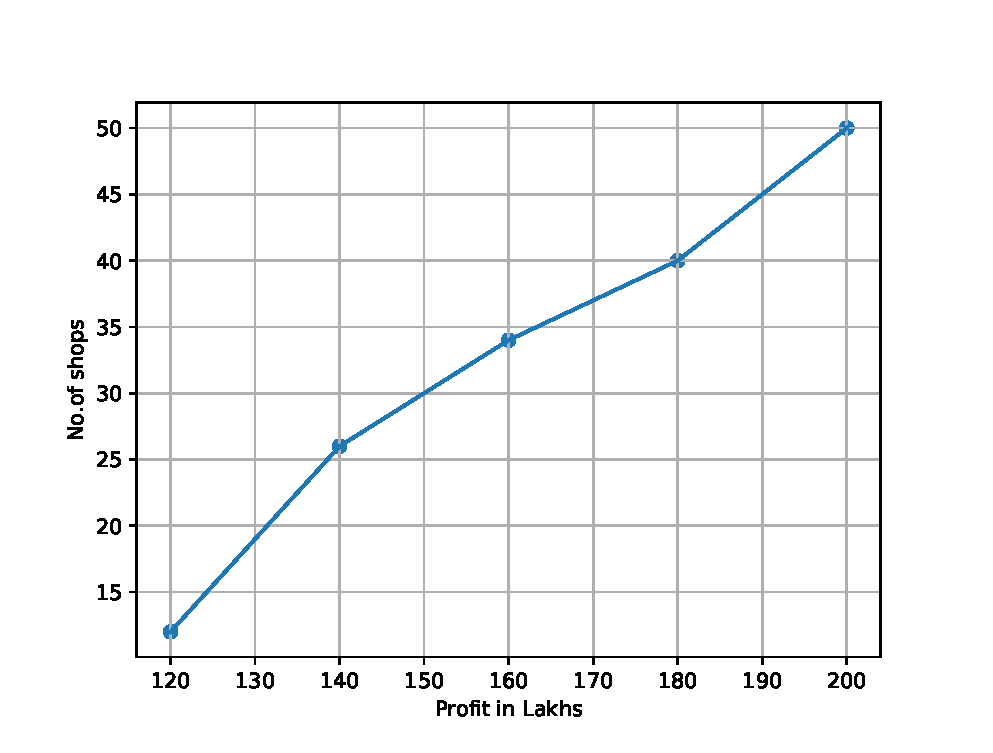
\includegraphics[width=\columnwidth]{./solutions/20-30/figs/statistics/exercises/ex_q23.eps}
	\caption{Ogive of Q.23}
	\label{fig:q23_ogive}	
	\end{figure}
	
	\begin{table}[ht]
	\begin{center}
    	%%%%%%%%%%%%%%%%%%%%%%%%%%%%%%%%%%%%%%%%%%%%%%%%%%%%%%%%%%%%%%%%%%%%%%
%%                                                                  %%
%%  This is the header of a LaTeX2e file exported from Gnumeric.    %%
%%                                                                  %%
%%  This file can be compiled as it stands or included in another   %%
%%  LaTeX document. The table is based on the longtable package so  %%
%%  the longtable options (headers, footers...) can be set in the   %%
%%  preamble section below (see PRAMBLE).                           %%
%%                                                                  %%
%%  To include the file in another, the following two lines must be %%
%%  in the including file:                                          %%
%%        \def\inputGnumericTable{}                                 %%
%%  at the beginning of the file and:                               %%
%%        \input{name-of-this-file.tex}                             %%
%%  where the table is to be placed. Note also that the including   %%
%%  file must use the following packages for the table to be        %%
%%  rendered correctly:                                             %%
%%    \usepackage[latin1]{inputenc}                                 %%
%%    \usepackage{color}                                            %%
%%    \usepackage{array}                                            %%
%%    \usepackage{longtable}                                        %%
%%    \usepackage{calc}                                             %%
%%    \usepackage{multirow}                                         %%
%%    \usepackage{hhline}                                           %%
%%    \usepackage{ifthen}                                           %%
%%  optionally (for landscape tables embedded in another document): %%
%%    \usepackage{lscape}                                           %%
%%                                                                  %%
%%%%%%%%%%%%%%%%%%%%%%%%%%%%%%%%%%%%%%%%%%%%%%%%%%%%%%%%%%%%%%%%%%%%%%



%%  This section checks if we are begin input into another file or  %%
%%  the file will be compiled alone. First use a macro taken from   %%
%%  the TeXbook ex 7.7 (suggestion of Han-Wen Nienhuys).            %%
\def\ifundefined#1{\expandafter\ifx\csname#1\endcsname\relax}


%%  Check for the \def token for inputed files. If it is not        %%
%%  defined, the file will be processed as a standalone and the     %%
%%  preamble will be used.                                          %%
\ifundefined{inputGnumericTable}

%%  We must be able to close or not the document at the end.        %%
	\def\gnumericTableEnd{\end{document}}


%%%%%%%%%%%%%%%%%%%%%%%%%%%%%%%%%%%%%%%%%%%%%%%%%%%%%%%%%%%%%%%%%%%%%%
%%                                                                  %%
%%  This is the PREAMBLE. Change these values to get the right      %%
%%  paper size and other niceties.                                  %%
%%                                                                  %%
%%%%%%%%%%%%%%%%%%%%%%%%%%%%%%%%%%%%%%%%%%%%%%%%%%%%%%%%%%%%%%%%%%%%%%

	\documentclass[12pt%
			  %,landscape%
                    ]{report}
       \usepackage[latin1]{inputenc}
       \usepackage{fullpage}
       \usepackage{color}
       \usepackage{array}
       \usepackage{longtable}
       \usepackage{calc}
       \usepackage{multirow}
       \usepackage{hhline}
       \usepackage{ifthen}

	\begin{document}


%%  End of the preamble for the standalone. The next section is for %%
%%  documents which are included into other LaTeX2e files.          %%
\else

%%  We are not a stand alone document. For a regular table, we will %%
%%  have no preamble and only define the closing to mean nothing.   %%
    \def\gnumericTableEnd{}

%%  If we want landscape mode in an embedded document, comment out  %%
%%  the line above and uncomment the two below. The table will      %%
%%  begin on a new page and run in landscape mode.                  %%
%       \def\gnumericTableEnd{\end{landscape}}
%       \begin{landscape}


%%  End of the else clause for this file being \input.              %%
\fi

%%%%%%%%%%%%%%%%%%%%%%%%%%%%%%%%%%%%%%%%%%%%%%%%%%%%%%%%%%%%%%%%%%%%%%
%%                                                                  %%
%%  The rest is the gnumeric table, except for the closing          %%
%%  statement. Changes below will alter the table's appearance.     %%
%%                                                                  %%
%%%%%%%%%%%%%%%%%%%%%%%%%%%%%%%%%%%%%%%%%%%%%%%%%%%%%%%%%%%%%%%%%%%%%%

\providecommand{\gnumericmathit}[1]{#1} 
%%  Uncomment the next line if you would like your numbers to be in %%
%%  italics if they are italizised in the gnumeric table.           %%
%\renewcommand{\gnumericmathit}[1]{\mathit{#1}}
\providecommand{\gnumericPB}[1]%
{\let\gnumericTemp=\\#1\let\\=\gnumericTemp\hspace{0pt}}
 \ifundefined{gnumericTableWidthDefined}
        \newlength{\gnumericTableWidth}
        \newlength{\gnumericTableWidthComplete}
        \newlength{\gnumericMultiRowLength}
        \global\def\gnumericTableWidthDefined{}
 \fi
%% The following setting protects this code from babel shorthands.  %%
 \ifthenelse{\isundefined{\languageshorthands}}{}{\languageshorthands{english}}
%%  The default table format retains the relative column widths of  %%
%%  gnumeric. They can easily be changed to c, r or l. In that case %%
%%  you may want to comment out the next line and uncomment the one %%
%%  thereafter                                                      %%
\providecommand\gnumbox{\makebox[0pt]}
%%\providecommand\gnumbox[1][]{\makebox}

%% to adjust positions in multirow situations                       %%
\setlength{\bigstrutjot}{\jot}
\setlength{\extrarowheight}{\doublerulesep}

%%  The \setlongtables command keeps column widths the same across  %%
%%  pages. Simply comment out next line for varying column widths.  %%
\setlongtables

\setlength\gnumericTableWidth{%
	70pt+%
	40pt+%
	53pt+%
0pt}
\def\gumericNumCols{3}
\setlength\gnumericTableWidthComplete{\gnumericTableWidth+%
         \tabcolsep*\gumericNumCols*2+\arrayrulewidth*\gumericNumCols}
\ifthenelse{\lengthtest{\gnumericTableWidthComplete > \linewidth}}%
         {\def\gnumericScale{\ratio{\linewidth-%
                        \tabcolsep*\gumericNumCols*2-%
                        \arrayrulewidth*\gumericNumCols}%
{\gnumericTableWidth}}}%
{\def\gnumericScale{1}}

%%%%%%%%%%%%%%%%%%%%%%%%%%%%%%%%%%%%%%%%%%%%%%%%%%%%%%%%%%%%%%%%%%%%%%
%%                                                                  %%
%% The following are the widths of the various columns. We are      %%
%% defining them here because then they are easier to change.       %%
%% Depending on the cell formats we may use them more than once.    %%
%%                                                                  %%
%%%%%%%%%%%%%%%%%%%%%%%%%%%%%%%%%%%%%%%%%%%%%%%%%%%%%%%%%%%%%%%%%%%%%%

\ifthenelse{\isundefined{\gnumericColA}}{\newlength{\gnumericColA}}{}\settowidth{\gnumericColA}{\begin{tabular}{@{}p{70pt*\gnumericScale}@{}}x\end{tabular}}
\ifthenelse{\isundefined{\gnumericColB}}{\newlength{\gnumericColB}}{}\settowidth{\gnumericColB}{\begin{tabular}{@{}p{40pt*\gnumericScale}@{}}x\end{tabular}}
\ifthenelse{\isundefined{\gnumericColC}}{\newlength{\gnumericColC}}{}\settowidth{\gnumericColC}{\begin{tabular}{@{}p{53pt*\gnumericScale}@{}}x\end{tabular}}

\begin{tabular}[c]{%
	b{\gnumericColA}%
	b{\gnumericColB}%
	b{\gnumericColC}%
	}

%%%%%%%%%%%%%%%%%%%%%%%%%%%%%%%%%%%%%%%%%%%%%%%%%%%%%%%%%%%%%%%%%%%%%%
%%  The longtable options. (Caption, headers... see Goosens, p.124) %%
%	\caption{The Table Caption.}             \\	%
% \hline	% Across the top of the table.
%%  The rest of these options are table rows which are placed on    %%
%%  the first, last or every page. Use \multicolumn if you want.    %%

%%  Header for the first page.                                      %%
%	\multicolumn{3}{c}{The First Header} \\ \hline 
%	\multicolumn{1}{c}{colTag}	%Column 1
%	&\multicolumn{1}{c}{colTag}	%Column 2
%	&\multicolumn{1}{c}{colTag}	\\ \hline %Last column
%	\endfirsthead

%%  The running header definition.                                  %%
%	\hline
%	\multicolumn{3}{l}{\ldots\small\slshape continued} \\ \hline
%	\multicolumn{1}{c}{colTag}	%Column 1
%	&\multicolumn{1}{c}{colTag}	%Column 2
%	&\multicolumn{1}{c}{colTag}	\\ \hline %Last column
%	\endhead

%%  The running footer definition.                                  %%
%	\hline
%	\multicolumn{3}{r}{\small\slshape continued\ldots} \\
%	\endfoot

%%  The ending footer definition.                                   %%
%	\multicolumn{3}{c}{That's all folks} \\ \hline 
%	\endlastfoot
%%%%%%%%%%%%%%%%%%%%%%%%%%%%%%%%%%%%%%%%%%%%%%%%%%%%%%%%%%%%%%%%%%%%%%

\hhline{|-|-~}
	 \multicolumn{1}{|p{\gnumericColA}|}%
	{\gnumericPB{\raggedright}\gnumbox[l]{wages}}
	&\multicolumn{1}{p{\gnumericColB}|}%
	{\gnumericPB{\raggedright}\gnumbox[l]{workers}}
	&
\\
\hhline{|--|~}
	 \multicolumn{1}{|p{\gnumericColA}|}%
	{\gnumericPB{\raggedright}\gnumbox[l]{Less than 120}}
	&\multicolumn{1}{p{\gnumericColB}|}%
	{\gnumericPB{\raggedright}\gnumbox[l]{12}}
	&
\\
\hhline{|--|~}
	 \multicolumn{1}{|p{\gnumericColA}|}%
	{\gnumericPB{\raggedright}\gnumbox[l]{Less than 140}}
	&\multicolumn{1}{p{\gnumericColB}|}%
	{\gnumericPB{\raggedright}\gnumbox[l]{26}}
	&
\\
\hhline{|--|~}
	 \multicolumn{1}{|p{\gnumericColA}|}%
	{\gnumericPB{\raggedright}\gnumbox[l]{Less than 160}}
	&\multicolumn{1}{p{\gnumericColB}|}%
	{\gnumericPB{\raggedright}\gnumbox[l]{34}}
	&
\\
\hhline{|--|~}
	 \multicolumn{1}{|p{\gnumericColA}|}%
	{\gnumericPB{\raggedright}\gnumbox[l]{Less than 180}}
	&\multicolumn{1}{p{\gnumericColB}|}%
	{\gnumericPB{\raggedright}\gnumbox[l]{40}}
	&
\\
\hhline{|--|~}
	 \multicolumn{1}{|p{\gnumericColA}|}%
	{\gnumericPB{\raggedright}\gnumbox[l]{Less than 200}}
	&\multicolumn{1}{p{\gnumericColB}|}%
	{\gnumericPB{\raggedright}\gnumbox[l]{50}}
	&
\\
\hhline{|-|-|~}
\end{tabular}

\ifthenelse{\isundefined{\languageshorthands}}{}{\languageshorthands{\languagename}}
\gnumericTableEnd

	\caption{Wages obtained using less than cumulative frequency}
	\label{table:table3}
	\end{center}
	\end{table}



\item If A and B are two independent events, then the probability of occurrence of at least one of A and B is given by 1- $P(A^{'}) P(B^{'})$\\
\solution
The following python code computes the median .
	\begin{lstlisting}
	codes/statistics/exercises/q24.py
	\end{lstlisting}
	
	
	\begin{align}
	\text{Median} &= l + \frac{\frac{n}{2} -cf}{f}\times h
	\end{align}
	\begin{align}
	\text{n} = \sum f_{i} = 100 \implies \frac{n}{2} = 50\\
	\end{align}
	$\therefore$ 46-48 is the median class.\\
	Here l is the lower limit of the median class = 46\\
	h is the classinterval =2\\
	cf is the cumulative frequency of the class before median class = 14\\
	f is the frequency of the median class =14

	\begin{align}
	\text{Median} &= 46 + \frac{17.5 - 14}{14}\times 2\\
	\text{Median} &= 46 + 0.5 = 46.5
	\end{align}
	Hence median weight is 46.5
	\begin{table}[ht]
	\begin{center}
    	%%%%%%%%%%%%%%%%%%%%%%%%%%%%%%%%%%%%%%%%%%%%%%%%%%%%%%%%%%%%%%%%%%%%%%
%%                                                                  %%
%%  This is the header of a LaTeX2e file exported from Gnumeric.    %%
%%                                                                  %%
%%  This file can be compiled as it stands or included in another   %%
%%  LaTeX document. The table is based on the longtable package so  %%
%%  the longtable options (headers, footers...) can be set in the   %%
%%  preamble section below (see PRAMBLE).                           %%
%%                                                                  %%
%%  To include the file in another, the following two lines must be %%
%%  in the including file:                                          %%
%%        \def\inputGnumericTable{}                                 %%
%%  at the beginning of the file and:                               %%
%%        \input{name-of-this-file.tex}                             %%
%%  where the table is to be placed. Note also that the including   %%
%%  file must use the following packages for the table to be        %%
%%  rendered correctly:                                             %%
%%    \usepackage[latin1]{inputenc}                                 %%
%%    \usepackage{color}                                            %%
%%    \usepackage{array}                                            %%
%%    \usepackage{longtable}                                        %%
%%    \usepackage{calc}                                             %%
%%    \usepackage{multirow}                                         %%
%%    \usepackage{hhline}                                           %%
%%    \usepackage{ifthen}                                           %%
%%  optionally (for landscape tables embedded in another document): %%
%%    \usepackage{lscape}                                           %%
%%                                                                  %%
%%%%%%%%%%%%%%%%%%%%%%%%%%%%%%%%%%%%%%%%%%%%%%%%%%%%%%%%%%%%%%%%%%%%%%



%%  This section checks if we are begin input into another file or  %%
%%  the file will be compiled alone. First use a macro taken from   %%
%%  the TeXbook ex 7.7 (suggestion of Han-Wen Nienhuys).            %%
\def\ifundefined#1{\expandafter\ifx\csname#1\endcsname\relax}


%%  Check for the \def token for inputed files. If it is not        %%
%%  defined, the file will be processed as a standalone and the     %%
%%  preamble will be used.                                          %%
\ifundefined{inputGnumericTable}

%%  We must be able to close or not the document at the end.        %%
	\def\gnumericTableEnd{\end{document}}


%%%%%%%%%%%%%%%%%%%%%%%%%%%%%%%%%%%%%%%%%%%%%%%%%%%%%%%%%%%%%%%%%%%%%%
%%                                                                  %%
%%  This is the PREAMBLE. Change these values to get the right      %%
%%  paper size and other niceties.                                  %%
%%                                                                  %%
%%%%%%%%%%%%%%%%%%%%%%%%%%%%%%%%%%%%%%%%%%%%%%%%%%%%%%%%%%%%%%%%%%%%%%

	\documentclass[12pt%
			  %,landscape%
                    ]{report}
       \usepackage[latin1]{inputenc}
       \usepackage{fullpage}
       \usepackage{color}
       \usepackage{array}
       \usepackage{longtable}
       \usepackage{calc}
       \usepackage{multirow}
       \usepackage{hhline}
       \usepackage{ifthen}

	\begin{document}


%%  End of the preamble for the standalone. The next section is for %%
%%  documents which are included into other LaTeX2e files.          %%
\else

%%  We are not a stand alone document. For a regular table, we will %%
%%  have no preamble and only define the closing to mean nothing.   %%
    \def\gnumericTableEnd{}

%%  If we want landscape mode in an embedded document, comment out  %%
%%  the line above and uncomment the two below. The table will      %%
%%  begin on a new page and run in landscape mode.                  %%
%       \def\gnumericTableEnd{\end{landscape}}
%       \begin{landscape}


%%  End of the else clause for this file being \input.              %%
\fi

%%%%%%%%%%%%%%%%%%%%%%%%%%%%%%%%%%%%%%%%%%%%%%%%%%%%%%%%%%%%%%%%%%%%%%
%%                                                                  %%
%%  The rest is the gnumeric table, except for the closing          %%
%%  statement. Changes below will alter the table's appearance.     %%
%%                                                                  %%
%%%%%%%%%%%%%%%%%%%%%%%%%%%%%%%%%%%%%%%%%%%%%%%%%%%%%%%%%%%%%%%%%%%%%%

\providecommand{\gnumericmathit}[1]{#1} 
%%  Uncomment the next line if you would like your numbers to be in %%
%%  italics if they are italizised in the gnumeric table.           %%
%\renewcommand{\gnumericmathit}[1]{\mathit{#1}}
\providecommand{\gnumericPB}[1]%
{\let\gnumericTemp=\\#1\let\\=\gnumericTemp\hspace{0pt}}
 \ifundefined{gnumericTableWidthDefined}
        \newlength{\gnumericTableWidth}
        \newlength{\gnumericTableWidthComplete}
        \newlength{\gnumericMultiRowLength}
        \global\def\gnumericTableWidthDefined{}
 \fi
%% The following setting protects this code from babel shorthands.  %%
 \ifthenelse{\isundefined{\languageshorthands}}{}{\languageshorthands{english}}
%%  The default table format retains the relative column widths of  %%
%%  gnumeric. They can easily be changed to c, r or l. In that case %%
%%  you may want to comment out the next line and uncomment the one %%
%%  thereafter                                                      %%
\providecommand\gnumbox{\makebox[0pt]}
%%\providecommand\gnumbox[1][]{\makebox}

%% to adjust positions in multirow situations                       %%
\setlength{\bigstrutjot}{\jot}
\setlength{\extrarowheight}{\doublerulesep}

%%  The \setlongtables command keeps column widths the same across  %%
%%  pages. Simply comment out next line for varying column widths.  %%
\setlongtables

\setlength\gnumericTableWidth{%
	53pt+%
	53pt+%
	53pt+%
0pt}
\def\gumericNumCols{3}
\setlength\gnumericTableWidthComplete{\gnumericTableWidth+%
         \tabcolsep*\gumericNumCols*2+\arrayrulewidth*\gumericNumCols}
\ifthenelse{\lengthtest{\gnumericTableWidthComplete > \linewidth}}%
         {\def\gnumericScale{\ratio{\linewidth-%
                        \tabcolsep*\gumericNumCols*2-%
                        \arrayrulewidth*\gumericNumCols}%
{\gnumericTableWidth}}}%
{\def\gnumericScale{1}}

%%%%%%%%%%%%%%%%%%%%%%%%%%%%%%%%%%%%%%%%%%%%%%%%%%%%%%%%%%%%%%%%%%%%%%
%%                                                                  %%
%% The following are the widths of the various columns. We are      %%
%% defining them here because then they are easier to change.       %%
%% Depending on the cell formats we may use them more than once.    %%
%%                                                                  %%
%%%%%%%%%%%%%%%%%%%%%%%%%%%%%%%%%%%%%%%%%%%%%%%%%%%%%%%%%%%%%%%%%%%%%%

\ifthenelse{\isundefined{\gnumericColA}}{\newlength{\gnumericColA}}{}\settowidth{\gnumericColA}{\begin{tabular}{@{}p{53pt*\gnumericScale}@{}}x\end{tabular}}
\ifthenelse{\isundefined{\gnumericColB}}{\newlength{\gnumericColB}}{}\settowidth{\gnumericColB}{\begin{tabular}{@{}p{53pt*\gnumericScale}@{}}x\end{tabular}}
\ifthenelse{\isundefined{\gnumericColC}}{\newlength{\gnumericColC}}{}\settowidth{\gnumericColC}{\begin{tabular}{@{}p{53pt*\gnumericScale}@{}}x\end{tabular}}

\begin{tabular}[c]{%
	b{\gnumericColA}%
	b{\gnumericColB}%
	b{\gnumericColC}%
	}

%%%%%%%%%%%%%%%%%%%%%%%%%%%%%%%%%%%%%%%%%%%%%%%%%%%%%%%%%%%%%%%%%%%%%%
%%  The longtable options. (Caption, headers... see Goosens, p.124) %%
%	\caption{The Table Caption.}             \\	%
% \hline	% Across the top of the table.
%%  The rest of these options are table rows which are placed on    %%
%%  the first, last or every page. Use \multicolumn if you want.    %%

%%  Header for the first page.                                      %%
%	\multicolumn{3}{c}{The First Header} \\ \hline 
%	\multicolumn{1}{c}{colTag}	%Column 1
%	&\multicolumn{1}{c}{colTag}	%Column 2
%	&\multicolumn{1}{c}{colTag}	\\ \hline %Last column
%	\endfirsthead

%%  The running header definition.                                  %%
%	\hline
%	\multicolumn{3}{l}{\ldots\small\slshape continued} \\ \hline
%	\multicolumn{1}{c}{colTag}	%Column 1
%	&\multicolumn{1}{c}{colTag}	%Column 2
%	&\multicolumn{1}{c}{colTag}	\\ \hline %Last column
%	\endhead

%%  The running footer definition.                                  %%
%	\hline
%	\multicolumn{3}{r}{\small\slshape continued\ldots} \\
%	\endfoot

%%  The ending footer definition.                                   %%
%	\multicolumn{3}{c}{That's all folks} \\ \hline 
%	\endlastfoot
%%%%%%%%%%%%%%%%%%%%%%%%%%%%%%%%%%%%%%%%%%%%%%%%%%%%%%%%%%%%%%%%%%%%%%

\hhline{|-|-|-}
	 \multicolumn{1}{|p{\gnumericColA}|}%
	{\gnumericPB{\raggedright}\gnumbox[l]{weight}}
	&\multicolumn{1}{p{\gnumericColB}|}%
	{\gnumericPB{\raggedright}\gnumbox[l]{No.of.student}}
	&\multicolumn{1}{p{\gnumericColC}|}%
	{\gnumericPB{\raggedright}\gnumbox[l]{Cum.Freq}}
\\
\hhline{|---|}
	 \multicolumn{1}{|p{\gnumericColA}|}%
	{\gnumericPB{\raggedright}\gnumbox[l]{0-38}}
	&\multicolumn{1}{p{\gnumericColB}|}%
	{\gnumericPB{\raggedright}\gnumbox[l]{0}}
	&\multicolumn{1}{p{\gnumericColC}|}%
	{\gnumericPB{\raggedright}\gnumbox[l]{0}}
\\
\hhline{|---|}
	 \multicolumn{1}{|p{\gnumericColA}|}%
	{\gnumericPB{\raggedright}\gnumbox[l]{38-40}}
	&\multicolumn{1}{p{\gnumericColB}|}%
	{\gnumericPB{\raggedright}\gnumbox[l]{3}}
	&\multicolumn{1}{p{\gnumericColC}|}%
	{\gnumericPB{\raggedright}\gnumbox[l]{3}}
\\
\hhline{|---|}
	 \multicolumn{1}{|p{\gnumericColA}|}%
	{\gnumericPB{\raggedright}\gnumbox[l]{40-42}}
	&\multicolumn{1}{p{\gnumericColB}|}%
	{\gnumericPB{\raggedright}\gnumbox[l]{2}}
	&\multicolumn{1}{p{\gnumericColC}|}%
	{\gnumericPB{\raggedright}\gnumbox[l]{5}}
\\
\hhline{|---|}
	 \multicolumn{1}{|p{\gnumericColA}|}%
	{\gnumericPB{\raggedright}\gnumbox[l]{42-44}}
	&\multicolumn{1}{p{\gnumericColB}|}%
	{\gnumericPB{\raggedright}\gnumbox[l]{4}}
	&\multicolumn{1}{p{\gnumericColC}|}%
	{\gnumericPB{\raggedright}\gnumbox[l]{9}}
\\
\hhline{|---|}
	 \multicolumn{1}{|p{\gnumericColA}|}%
	{\gnumericPB{\raggedright}\gnumbox[l]{44-46}}
	&\multicolumn{1}{p{\gnumericColB}|}%
	{\gnumericPB{\raggedright}\gnumbox[l]{5}}
	&\multicolumn{1}{p{\gnumericColC}|}%
	{\gnumericPB{\raggedright}\gnumbox[l]{14}}
\\
\hhline{|---|}
	 \multicolumn{1}{|p{\gnumericColA}|}%
	{\gnumericPB{\raggedright}\gnumbox[l]{46-48}}
	&\multicolumn{1}{p{\gnumericColB}|}%
	{\gnumericPB{\raggedright}\gnumbox[l]{14}}
	&\multicolumn{1}{p{\gnumericColC}|}%
	{\gnumericPB{\raggedright}\gnumbox[l]{28}}
\\
\hhline{|---|}
	 \multicolumn{1}{|p{\gnumericColA}|}%
	{\gnumericPB{\raggedright}\gnumbox[l]{48-50}}
	&\multicolumn{1}{p{\gnumericColB}|}%
	{\gnumericPB{\raggedright}\gnumbox[l]{4}}
	&\multicolumn{1}{p{\gnumericColC}|}%
	{\gnumericPB{\raggedright}\gnumbox[l]{32}}
\\
\hhline{|---|}
	 \multicolumn{1}{|p{\gnumericColA}|}%
	{\gnumericPB{\raggedright}\gnumbox[l]{50-52}}
	&\multicolumn{1}{p{\gnumericColB}|}%
	{\gnumericPB{\raggedright}\gnumbox[l]{3}}
	&\multicolumn{1}{p{\gnumericColC}|}%
	{\gnumericPB{\raggedright}\gnumbox[l]{35}}
\\
\hhline{|-|-|-|}
\end{tabular}

\ifthenelse{\isundefined{\languageshorthands}}{}{\languageshorthands{\languagename}}
\gnumericTableEnd

	\caption{Frequency distribution of the weights of students}
	\label{table:stat_ex_q24_anstable10}
	\end{center}
	\end{table}


\item Given that $E$ and $F$ are events such that $\pr{E} = 0.6, \pr{F} = 0.3$ and $\pr{EF} = 0.2$, find $\pr{E|F}$ and $\pr{F|E}$.\\
\solution
By definition, 
\begin{align}
\pr{A|B} = \frac{\pr{AB}}{\pr{B}}
\end{align}
Thus, we can write:
\begin{align}
\pr{E|F} = \frac{\pr{EF}}{\pr{F}} = \frac{0.2}{0.3} = \frac{2}{3}
\end{align}
In a similar manner:
\begin{align}
\pr{F|E} = \frac{\pr{EF}}{\pr{E}} = \frac{0.2}{0.6} = \frac{1}{3}
\end{align}
%
\item Compute P(A/B), if P(B) = 0.5 and P (A $\cap$ B) = 0.32.\\
\solution
For two events A and B, by definition,
\begin{align}
\pr{A|B} = \frac{\pr{AB}}{\pr{B}}
\end{align}
Given $\pr{B} = 0.5$ and $\pr{AB} = 0.32$
\begin{align}
\pr{A | B} = \frac{0.32}{0.5}
\end{align}
Thus,
\begin{align}
\pr{A | B} = 0.64
\end{align}

\item If P(A) = 0.8, P(B) = 0.5 and P(B/A) = 0.4, find\\
(i) P(A $\cap$ B)\\
(ii) P(A/B)\\ 
(iii) P(A $\cup$ B)\\
\solution
 \begin{enumerate}
\item By the definition
\begin{align}
\Pr\brak{B/A} = \frac{\Pr\brak{AB}}{\Pr\brak{A}}
\end{align}
Substituting the values,
\begin{align}
\Pr\brak{AB} = \frac{2}{5} \times \frac{4}{5}\\
\Pr\brak{AB} = \frac{8}{25}
\end{align}
\item By the definition
\begin{align}
\Pr\brak{A/B} = \frac{\Pr\brak{AB}}{\Pr\brak{B}}
\end{align}
Substituting the values,
\begin{align}
\Pr\brak{A/B} = \frac {\frac{8}{25}} {\frac{1}{2}}\\
\Pr\brak{A/B} = \frac{16}{25}
\end{align}
\item By the result
\begin{align}
\Pr\brak{A+B} = \Pr\brak{A} + \Pr\brak{B} - \Pr\brak{AB}
\end{align}
Substituting the values,
\begin{align}
\Pr\brak{A+B} = \frac{4}{5} + \frac{1}{2} - \frac{8}{25}\\
\Pr\brak{A+B} = \frac{98}{100}
\end{align}
\end{enumerate}
\item Evaluate P(A $\cup$ B), if 2P(A) = P(B)  = $\frac{5}{13}$ and P(A/B) =  $\frac{2}{5}.$\\
\solution
By definition,
\begin{align}
\Pr\brak{A/B} = \frac{\Pr\brak{AB}}{\Pr\brak{B}}
\end{align}
Substituting the values,
\begin{align}
\frac{2}{5} = \frac{\Pr\brak{AB}}{5/13}\\
 \Pr\brak{AB} = \frac{2}{13}
\end{align}
\begin{align}
\Pr\brak{A+B} = \Pr\brak{A} + \Pr\brak{B} - \Pr\brak{AB}
\end{align}
Substituting the values,
\begin{align}
\Pr\brak{A+B} = \frac{5}{26} + \frac{5}{13} - \frac{2}{13} = \frac{11}{26}
\end{align}

\item If P(A) = $\frac{6}{11}$, P(B) = $\frac{5}{11}$ and P(A $\cup$ B) = $\frac{11}{7}$ find\\
(i) P(A $\cap$ B)\\ 
(ii) P(A/B)\\ 
(iii) P(B/A)
\\
\solution 
\begin{enumerate}
\item 
\begin{align}
\pr{A + B} = \pr{A} + \pr{B} - \pr{AB}
\end{align}
Substituting the values,
\begin{align}
\frac{7}{11} = \frac{6}{11} + \frac{5}{11} - \pr{AB}\\
 \pr{AB} = 1 - \frac{7}{11} = \frac{4}{11}
\end{align}
\item
\begin{align}
\pr{A|B} = \frac{\pr{AB}}{\pr{B}} = \frac{4/11}{5/11} = \frac{4}{5}
\end{align}
\item
\begin{align}
\pr{B|A} = \frac{\pr{AB}}{\pr{A}} = \frac{4/11}{6/11} = \frac{2}{3}
\end{align}
\end{enumerate}
\item A fair die is rolled. Consider the events E =  (1, 3, 5), F = (2, 3) and G = (2, 3, 4, 5) Find\\
(i) P(E/F) and P(F/E) \\
(ii) P(E/G) and P(G/E)\\
(iii) P((E $\cup$ F)/G) and P((E $\cap$ F)/G)\\
\solution
From the given information,
	\begin{align}
	\pr{E} &= \frac{3}{6} = \frac{1}{2} \\
	\pr{F} &= \frac{2}{6} = \frac{1}{3} \\	
	\pr{G} &= \frac{4}{6} = \frac{2}{3} \\	
	\pr{E F} &= \frac{1}{6}\\
	\pr{E G} &= \frac{2}{6}= \frac{1}{3}\\
	\pr{F G} &= \frac{2}{6}= \frac{1}{3}\\
	\pr{E F G} &= \frac{1}{6}
\end{align}
\begin{enumerate}
\item	
\begin{align}
	\pr{E|F} &= \frac{\pr{E F}}{\pr{F}}\\
	\pr{E|F} &= \frac{\frac{1}{6}}{\frac{1}{3}} = \frac{1}{2}\\
	\pr{F|E} &= \frac{\pr{F E}}{\pr{E}}\\
	\pr{F|E} &= \frac{\frac{1}{6}}{\frac{1}{2}} = \frac{1}{3}
	\end{align}

\item 	\begin{align}
	\pr{E|G} &= \frac{\pr{E G}}{\pr{G}}\\
	\pr{E|G} &= \frac{\frac{1}{3}}{\frac{2}{3}} = \frac{1}{2}\\
	\pr{G|E} &= \frac{\pr{G E}}{\pr{G}}\\
	\pr{G|E} &= \frac{\frac{1}{3}}{\frac{1}{2}} = \frac{2}{3}\\
	\end{align}
	
\item	%$\pr{\frac{E\cup F}{G}}$
\begin{multline}
\pr{E+F|G} = \frac{\pr{\cbrak{E+F}G}}{\pr{G}}
\\
 = \frac{\pr{EG + FG}}{\pr{G}}
\\
=\frac{\pr{EG} +\pr{ FG}- \pr{EFG}}{\pr{G}}
\\
 = \frac{3}{4}
\end{multline}
and 
\begin{align}
\pr{EF|G} = 
\frac{ \pr{EFG}}{\pr{G}}
 = \frac{1}{4}
\end{align}

\end{enumerate}

\item Choose the correct answer, if P(A) = $\frac{1}{2}$, P(B) = 0, then P(A/B) is
\begin{enumerate}
\item 0
\item $\frac{1}{2}$
\item not defined
\item 1
\end{enumerate}
\solution
\subsection{Problem}

\renewcommand{\theequation}{\theenumi}
\begin{enumerate}[label=\thesection.\arabic*.,ref=\thesection.\theenumi]
\numberwithin{equation}{enumi}
\item For the examples given in the previous question classify them as primary data or secondary data\\
\solution  Primary data is the data collected by ourselves and secondary data is the information gathered from other sources.
\begin{enumerate}
		\item Weights of students of a class - Primary
		\item No. of plants in a locality - Primary
		\item No. of boys and girls in a class - Primary
		\item Runs scored in a match - Secondary
		\item Rainfall in the city in the past decade - Secondary
\end{enumerate}
	
\end{enumerate}


\item If A and B are events such that P(A/B) = P(B/A), then
\begin{enumerate}
\item A $\subset$ B but A $\neq$ B
\item A = B
\item A $\cap$ B = $\phi$
\item P(A) = P(B)
\end{enumerate}
\solution
\begin{align}
\pr{A|B} &= \pr{B|A}\\
\implies \frac{\pr{AB}}{\pr{A}} &= \frac{\pr{AB}}{\pr{B}}\\
\implies \pr{AB} &= 0 \implies AB = 0
\\
\text{ or, } \pr{A} &= \pr{B}
\end{align}


\item If P(A) = $\frac{3}{5}$ and P(B) = $\frac{1}{5}$, find P (A $\cap$ B) if A and B are independent events.\\\solution
	  See Table 	\ref{table:stat_ex_q29_quetable6}.
Since the minimum =2 and maximum = 32, we take the intervals as 0-5,5-10 and so on upto 30-35. It can be observed that there are very few engineers whose homes are at more than or equal to 20km distance from their work place and most engineers have their workplace at distance of 0km to 15km from their homes.
	\begin{table}[ht]
	\begin{center}
    	%%%%%%%%%%%%%%%%%%%%%%%%%%%%%%%%%%%%%%%%%%%%%%%%%%%%%%%%%%%%%%%%%%%%%%
%%                                                                  %%
%%  This is the header of a LaTeX2e file exported from Gnumeric.    %%
%%                                                                  %%
%%  This file can be compiled as it stands or included in another   %%
%%  LaTeX document. The table is based on the longtable package so  %%
%%  the longtable options (headers, footers...) can be set in the   %%
%%  preamble section below (see PRAMBLE).                           %%
%%                                                                  %%
%%  To include the file in another, the following two lines must be %%
%%  in the including file:                                          %%
%%        \def\inputGnumericTable{}                                 %%
%%  at the beginning of the file and:                               %%
%%        \input{name-of-this-file.tex}                             %%
%%  where the table is to be placed. Note also that the including   %%
%%  file must use the following packages for the table to be        %%
%%  rendered correctly:                                             %%
%%    \usepackage[latin1]{inputenc}                                 %%
%%    \usepackage{color}                                            %%
%%    \usepackage{array}                                            %%
%%    \usepackage{longtable}                                        %%
%%    \usepackage{calc}                                             %%
%%    \usepackage{multirow}                                         %%
%%    \usepackage{hhline}                                           %%
%%    \usepackage{ifthen}                                           %%
%%  optionally (for landscape tables embedded in another document): %%
%%    \usepackage{lscape}                                           %%
%%                                                                  %%
%%%%%%%%%%%%%%%%%%%%%%%%%%%%%%%%%%%%%%%%%%%%%%%%%%%%%%%%%%%%%%%%%%%%%%



%%  This section checks if we are begin input into another file or  %%
%%  the file will be compiled alone. First use a macro taken from   %%
%%  the TeXbook ex 7.7 (suggestion of Han-Wen Nienhuys).            %%
\def\ifundefined#1{\expandafter\ifx\csname#1\endcsname\relax}


%%  Check for the \def token for inputed files. If it is not        %%
%%  defined, the file will be processed as a standalone and the     %%
%%  preamble will be used.                                          %%
\ifundefined{inputGnumericTable}

%%  We must be able to close or not the document at the end.        %%
	\def\gnumericTableEnd{\end{document}}


%%%%%%%%%%%%%%%%%%%%%%%%%%%%%%%%%%%%%%%%%%%%%%%%%%%%%%%%%%%%%%%%%%%%%%
%%                                                                  %%
%%  This is the PREAMBLE. Change these values to get the right      %%
%%  paper size and other niceties.                                  %%
%%                                                                  %%
%%%%%%%%%%%%%%%%%%%%%%%%%%%%%%%%%%%%%%%%%%%%%%%%%%%%%%%%%%%%%%%%%%%%%%

	\documentclass[12pt%
			  %,landscape%
                    ]{report}
       \usepackage[latin1]{inputenc}
       \usepackage{fullpage}
       \usepackage{color}
       \usepackage{array}
       \usepackage{longtable}
       \usepackage{calc}
       \usepackage{multirow}
       \usepackage{hhline}
       \usepackage{ifthen}

	\begin{document}


%%  End of the preamble for the standalone. The next section is for %%
%%  documents which are included into other LaTeX2e files.          %%
\else

%%  We are not a stand alone document. For a regular table, we will %%
%%  have no preamble and only define the closing to mean nothing.   %%
    \def\gnumericTableEnd{}

%%  If we want landscape mode in an embedded document, comment out  %%
%%  the line above and uncomment the two below. The table will      %%
%%  begin on a new page and run in landscape mode.                  %%
%       \def\gnumericTableEnd{\end{landscape}}
%       \begin{landscape}


%%  End of the else clause for this file being \input.              %%
\fi

%%%%%%%%%%%%%%%%%%%%%%%%%%%%%%%%%%%%%%%%%%%%%%%%%%%%%%%%%%%%%%%%%%%%%%
%%                                                                  %%
%%  The rest is the gnumeric table, except for the closing          %%
%%  statement. Changes below will alter the table's appearance.     %%
%%                                                                  %%
%%%%%%%%%%%%%%%%%%%%%%%%%%%%%%%%%%%%%%%%%%%%%%%%%%%%%%%%%%%%%%%%%%%%%%

\providecommand{\gnumericmathit}[1]{#1} 
%%  Uncomment the next line if you would like your numbers to be in %%
%%  italics if they are italizised in the gnumeric table.           %%
%\renewcommand{\gnumericmathit}[1]{\mathit{#1}}
\providecommand{\gnumericPB}[1]%
{\let\gnumericTemp=\\#1\let\\=\gnumericTemp\hspace{0pt}}
 \ifundefined{gnumericTableWidthDefined}
        \newlength{\gnumericTableWidth}
        \newlength{\gnumericTableWidthComplete}
        \newlength{\gnumericMultiRowLength}
        \global\def\gnumericTableWidthDefined{}
 \fi
%% The following setting protects this code from babel shorthands.  %%
 \ifthenelse{\isundefined{\languageshorthands}}{}{\languageshorthands{english}}
%%  The default table format retains the relative column widths of  %%
%%  gnumeric. They can easily be changed to c, r or l. In that case %%
%%  you may want to comment out the next line and uncomment the one %%
%%  thereafter                                                      %%
\providecommand\gnumbox{\makebox[0pt]}
%%\providecommand\gnumbox[1][]{\makebox}

%% to adjust positions in multirow situations                       %%
\setlength{\bigstrutjot}{\jot}
\setlength{\extrarowheight}{\doublerulesep}

%%  The \setlongtables command keeps column widths the same across  %%
%%  pages. Simply comment out next line for varying column widths.  %%
\setlongtables

\setlength\gnumericTableWidth{%
	53pt+%
	80pt+%
0pt}
\def\gumericNumCols{2}
\setlength\gnumericTableWidthComplete{\gnumericTableWidth+%
         \tabcolsep*\gumericNumCols*2+\arrayrulewidth*\gumericNumCols}
\ifthenelse{\lengthtest{\gnumericTableWidthComplete > \linewidth}}%
         {\def\gnumericScale{\ratio{\linewidth-%
                        \tabcolsep*\gumericNumCols*2-%
                        \arrayrulewidth*\gumericNumCols}%
{\gnumericTableWidth}}}%
{\def\gnumericScale{1}}

%%%%%%%%%%%%%%%%%%%%%%%%%%%%%%%%%%%%%%%%%%%%%%%%%%%%%%%%%%%%%%%%%%%%%%
%%                                                                  %%
%% The following are the widths of the various columns. We are      %%
%% defining them here because then they are easier to change.       %%
%% Depending on the cell formats we may use them more than once.    %%
%%                                                                  %%
%%%%%%%%%%%%%%%%%%%%%%%%%%%%%%%%%%%%%%%%%%%%%%%%%%%%%%%%%%%%%%%%%%%%%%

\ifthenelse{\isundefined{\gnumericColA}}{\newlength{\gnumericColA}}{}\settowidth{\gnumericColA}{\begin{tabular}{@{}p{53pt*\gnumericScale}@{}}x\end{tabular}}
\ifthenelse{\isundefined{\gnumericColB}}{\newlength{\gnumericColB}}{}\settowidth{\gnumericColB}{\begin{tabular}{@{}p{80pt*\gnumericScale}@{}}x\end{tabular}}

\begin{tabular}[c]{%
	b{\gnumericColA}%
	b{\gnumericColB}%
	}

%%%%%%%%%%%%%%%%%%%%%%%%%%%%%%%%%%%%%%%%%%%%%%%%%%%%%%%%%%%%%%%%%%%%%%
%%  The longtable options. (Caption, headers... see Goosens, p.124) %%
%	\caption{The Table Caption.}             \\	%
% \hline	% Across the top of the table.
%%  The rest of these options are table rows which are placed on    %%
%%  the first, last or every page. Use \multicolumn if you want.    %%

%%  Header for the first page.                                      %%
%	\multicolumn{2}{c}{The First Header} \\ \hline 
%	\multicolumn{1}{c}{colTag}	%Column 1
%	&\multicolumn{1}{c}{colTag}	\\ \hline %Last column
%	\endfirsthead

%%  The running header definition.                                  %%
%	\hline
%	\multicolumn{2}{l}{\ldots\small\slshape continued} \\ \hline
%	\multicolumn{1}{c}{colTag}	%Column 1
%	&\multicolumn{1}{c}{colTag}	\\ \hline %Last column
%	\endhead

%%  The running footer definition.                                  %%
%	\hline
%	\multicolumn{2}{r}{\small\slshape continued\ldots} \\
%	\endfoot

%%  The ending footer definition.                                   %%
%	\multicolumn{2}{c}{That's all folks} \\ \hline 
%	\endlastfoot
%%%%%%%%%%%%%%%%%%%%%%%%%%%%%%%%%%%%%%%%%%%%%%%%%%%%%%%%%%%%%%%%%%%%%%

\hhline{|-|-}
	 \multicolumn{1}{|p{\gnumericColA}|}%
	{\gnumericPB{\centering}\gnumbox{Distance(km)}}
	&\multicolumn{1}{p{\gnumericColB}|}%
	{\gnumericPB{\centering}\gnumbox{No.of.engineers}}
\\
\hhline{|--|}
	 \multicolumn{1}{|p{\gnumericColA}|}%
	{\gnumericPB{\centering}\gnumbox{0-5}}
	&\multicolumn{1}{p{\gnumericColB}|}%
	{\gnumericPB{\centering}\gnumbox{5}}
\\
\hhline{|--|}
	 \multicolumn{1}{|p{\gnumericColA}|}%
	{\gnumericPB{\centering}\gnumbox{005-10}}
	&\multicolumn{1}{p{\gnumericColB}|}%
	{\gnumericPB{\centering}\gnumbox{11}}
\\
\hhline{|--|}
	 \multicolumn{1}{|p{\gnumericColA}|}%
	{\gnumericPB{\centering}\gnumbox{10-15}}
	&\multicolumn{1}{p{\gnumericColB}|}%
	{\gnumericPB{\centering}\gnumbox{11}}
\\
\hhline{|--|}
	 \multicolumn{1}{|p{\gnumericColA}|}%
	{\gnumericPB{\centering}\gnumbox{15-20}}
	&\multicolumn{1}{p{\gnumericColB}|}%
	{\gnumericPB{\centering}\gnumbox{9}}
\\
\hhline{|--|}
	 \multicolumn{1}{|p{\gnumericColA}|}%
	{\gnumericPB{\centering}\gnumbox{20-25}}
	&\multicolumn{1}{p{\gnumericColB}|}%
	{\gnumericPB{\centering}\gnumbox{1}}
\\
\hhline{|--|}
	 \multicolumn{1}{|p{\gnumericColA}|}%
	{\gnumericPB{\centering}\gnumbox{25-30}}
	&\multicolumn{1}{p{\gnumericColB}|}%
	{\gnumericPB{\centering}\gnumbox{1}}
\\
\hhline{|--|}
	 \multicolumn{1}{|p{\gnumericColA}|}%
	{\gnumericPB{\centering}\gnumbox{30-35}}
	&\multicolumn{1}{p{\gnumericColB}|}%
	{\gnumericPB{\centering}\gnumbox{2}}
\\
\hhline{|--|}
	 \multicolumn{1}{|p{\gnumericColA}|}%
	{\gnumericPB{\centering}\gnumbox{Total}}
	&\multicolumn{1}{p{\gnumericColB}|}%
	{\gnumericPB{\centering}\gnumbox{40}}
\\
\hhline{|-|-|}
\end{tabular}

\ifthenelse{\isundefined{\languageshorthands}}{}{\languageshorthands{\languagename}}
\gnumericTableEnd

	\caption{distance of engineers from their residence to their place of work }
	\label{table:stat_ex_q29_quetable6}
	\end{center}
	\end{table}

	

\item One card is drawn at random from a well shuffled deck of 52 cards. In which of the following cases are the events E and F independent?\\
(i) E : 'the card drawn is a spade'
F : 'the card drawn is an ace'\\
(ii) E : 'the card drawn is black'
F : 'the card drawn is a king'\\
(iii) E : 'the card drawn is a king or queen'
F : 'the card drawn is a queen or jack'.\\
\solution
The given curve 
\begin{align}
	y =\frac{1}{x-1}
\end{align}
can be expressed as 
\begin{align}
	xy - y - 1 = 0 \label{eq:solutions/1/14/eq:hyperbola}
\end{align}
Hence, we have
\begin{align}
	\vec{V} = \frac{1}{2}\myvec{0 & 1 \\ 1 & 0}, 
	\vec{u} = \frac{1}{2}\myvec{0 \\-1},
	f = -1
\end{align}
Since $\mydet{\vec{V}} < 0$, the equation \eqref{eq:solutions/1/14/eq:hyperbola} represents hyperbola.
To find the values of $\lambda_1$ and $\lambda_2$, consider the characteristic equation,
\begin{align}
	\mydet{\lambda\vec{I} - \vec{V}} &= 0\\
	\implies \mydet{\myvec{\lambda & 0\\0 & \lambda} - \myvec{0 & \frac{1}{2} \\ \frac{1}{2} & 0}} &= 0\\
	\implies \mydet{ \lambda & \frac{-1}{2} \\ \frac{-1}{2} & \lambda} &= 0\\
	\implies \lambda_1 &= \frac{1}{2} , \lambda_2 = \frac{-1}{2}
\end{align}
In addition, given the slope -1, the direction and normal vectors are given by 
\begin{align}
	\vec{m} = \myvec{1 \\ -1} \\
	\vec{n} = \myvec{ 1 \\ 1}
\end{align}
The parameters of hyperbola are as follows:
\begin{align}
	\vec{c} &= -\vec{V}^{-1}\vec{u} \\
	&= -\myvec{0 & 2\\ 2 & 0}\myvec{0 \\ -\frac{1}{2}} \\
	&= \myvec{1 \\ 0}\\
	axes &= \begin{cases}
	\sqrt{\frac{\vec{u}^T\vec{V}^{-1}\vec{u} - f}{\lambda_1}} = \sqrt{2}\\
 \sqrt{\frac{f-\vec{u}^T\vec{V}^{-1}\vec{u}}{\lambda_2}} = \sqrt{2}
\end{cases}
\end{align}
which represents the standard hyperbola equation,
\begin{align}
	\frac{x^2}{2} - \frac{x^2}{2} = 1
\end{align}
The points of contact are given by 
\begin{align}
  \tiny{K} &=\pm \sqrt{\frac{\vec{u}^T\vec{V}^{-1}\vec{u} - f}{\vec{n}^T\vec{V}^{-1}\vec{n}}}
  = \pm \frac{1}{2}\\
  \vec{q} &= \vec{V}^{-1}(k\vec{n}-\vec{u})\\
  \vec{q_1} &= \myvec{0 & 2\\2 & 0} \sbrak{\frac{1}{2}\myvec{1 \\ 1} - \myvec{0\\ \frac{-1}{2}}}\\
  &= \myvec{2 \\ 1}\\
  \vec{q_2} &= \myvec{0 & 2\\2 & 0} \sbrak{\frac{-1}{2}\myvec{1 \\ 1} - \myvec{0\\ \frac{-1}{2}}}\\
  &= \myvec{0 \\ -1}
\end{align} 
$\therefore$ The tangents are given by
\begin{align}
	\myvec{1 & 1} \brak{\vec{x} - \myvec{2 \\ 1}} = 0 \\
	\myvec{1 & 1} \brak{\vec{x} - \myvec{0 \\ -1}} = 0
\end{align}
The desired equations of all lines having slope -1 that are tangents to the curve $\frac{1}{x-1}, x \neq 1$ are given by
\begin{align}
	\myvec{1 & 1}\vec{x} &= 3 \\
	\myvec{1 & 1}\vec{x} &= -1 
\end{align}
The above results are verified in the following figure.
\begin{figure}[h!] \label{eq:solutions/1/14/fig:tangents}
	\centering
	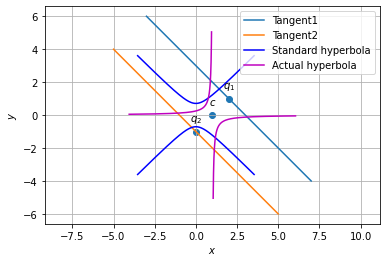
\includegraphics[width=\columnwidth]{./solutions/1/14/graph7.png}
	\caption{The standard and actual hyperbola.}
\end{figure}

\item Two events A and B will be independent, if
\begin{enumerate}
\item A and B are mutually exclusive
\item $P(A^{\prime}B^{\prime})$ = [1 – P(A)] [1 – P(B)]
\item P(A) = P(B)
\item P(A) + P(B) = 1
\end{enumerate}
\solution
The given curve 
\begin{align}
	y =\frac{1}{x-1}
\end{align}
can be expressed as 
\begin{align}
	xy - y - 1 = 0 \label{eq:solutions/1/14/eq:hyperbola}
\end{align}
Hence, we have
\begin{align}
	\vec{V} = \frac{1}{2}\myvec{0 & 1 \\ 1 & 0}, 
	\vec{u} = \frac{1}{2}\myvec{0 \\-1},
	f = -1
\end{align}
Since $\mydet{\vec{V}} < 0$, the equation \eqref{eq:solutions/1/14/eq:hyperbola} represents hyperbola.
To find the values of $\lambda_1$ and $\lambda_2$, consider the characteristic equation,
\begin{align}
	\mydet{\lambda\vec{I} - \vec{V}} &= 0\\
	\implies \mydet{\myvec{\lambda & 0\\0 & \lambda} - \myvec{0 & \frac{1}{2} \\ \frac{1}{2} & 0}} &= 0\\
	\implies \mydet{ \lambda & \frac{-1}{2} \\ \frac{-1}{2} & \lambda} &= 0\\
	\implies \lambda_1 &= \frac{1}{2} , \lambda_2 = \frac{-1}{2}
\end{align}
In addition, given the slope -1, the direction and normal vectors are given by 
\begin{align}
	\vec{m} = \myvec{1 \\ -1} \\
	\vec{n} = \myvec{ 1 \\ 1}
\end{align}
The parameters of hyperbola are as follows:
\begin{align}
	\vec{c} &= -\vec{V}^{-1}\vec{u} \\
	&= -\myvec{0 & 2\\ 2 & 0}\myvec{0 \\ -\frac{1}{2}} \\
	&= \myvec{1 \\ 0}\\
	axes &= \begin{cases}
	\sqrt{\frac{\vec{u}^T\vec{V}^{-1}\vec{u} - f}{\lambda_1}} = \sqrt{2}\\
 \sqrt{\frac{f-\vec{u}^T\vec{V}^{-1}\vec{u}}{\lambda_2}} = \sqrt{2}
\end{cases}
\end{align}
which represents the standard hyperbola equation,
\begin{align}
	\frac{x^2}{2} - \frac{x^2}{2} = 1
\end{align}
The points of contact are given by 
\begin{align}
  \tiny{K} &=\pm \sqrt{\frac{\vec{u}^T\vec{V}^{-1}\vec{u} - f}{\vec{n}^T\vec{V}^{-1}\vec{n}}}
  = \pm \frac{1}{2}\\
  \vec{q} &= \vec{V}^{-1}(k\vec{n}-\vec{u})\\
  \vec{q_1} &= \myvec{0 & 2\\2 & 0} \sbrak{\frac{1}{2}\myvec{1 \\ 1} - \myvec{0\\ \frac{-1}{2}}}\\
  &= \myvec{2 \\ 1}\\
  \vec{q_2} &= \myvec{0 & 2\\2 & 0} \sbrak{\frac{-1}{2}\myvec{1 \\ 1} - \myvec{0\\ \frac{-1}{2}}}\\
  &= \myvec{0 \\ -1}
\end{align} 
$\therefore$ The tangents are given by
\begin{align}
	\myvec{1 & 1} \brak{\vec{x} - \myvec{2 \\ 1}} = 0 \\
	\myvec{1 & 1} \brak{\vec{x} - \myvec{0 \\ -1}} = 0
\end{align}
The desired equations of all lines having slope -1 that are tangents to the curve $\frac{1}{x-1}, x \neq 1$ are given by
\begin{align}
	\myvec{1 & 1}\vec{x} &= 3 \\
	\myvec{1 & 1}\vec{x} &= -1 
\end{align}
The above results are verified in the following figure.
\begin{figure}[h!] \label{eq:solutions/1/14/fig:tangents}
	\centering
	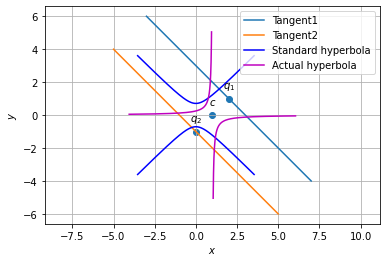
\includegraphics[width=\columnwidth]{./solutions/1/14/graph7.png}
	\caption{The standard and actual hyperbola.}
\end{figure}

\end{enumerate}

